\documentclass[sigplan,screen,review,natbib=true]{acmart}

%% The majority of ACM publications use class options [sigconf,review,anonymous].
%% For PLDI-adjacent workshops (like the E-Graphs Workshop), sigplan is appropriate.
%% Remove 'review' and 'anonymous' for the camera-ready version.

%% Rights management information.
\setcopyright{none}
\acmConference[EGRAPHS '26]{E-Graphs Workshop}{June 2026}{TBD}
\acmYear{2026}
\copyrightyear{2026}

%% Submission ID (remove for camera-ready).
% \acmSubmissionID{123-A56-BU3}

%% Remove ACM reference format for workshop submissions if desired.
\settopmatter{printacmref=false}
\renewcommand\footnotetextcopyrightpermission[1]{}
\pagestyle{plain}

%% Packages
\usepackage{booktabs}
\usepackage{subcaption}
\usepackage{stys/smtlib}

% Don't number subsubsections (acmart numbers them by default).
\setcounter{secnumdepth}{2}

\begin{document}

\title{Relational E-matching in an SMT solver}
% \subtitle{Optional Subtitle}

%% Author information. With 'anonymous' class option, these are hidden.
\author{Amar Shah}
\affiliation{%
  \institution{Carnegie Mellon University}
  \city{Pittsburgh}
  \country{USA}
}
\email{amarshah@andrew.cmu.edu}

\author{Marijn Heule}
\affiliation{%
  \institution{Carnegie Mellon University}
  \city{Pittsburgh}
  \country{USA}
}
\email{marijn@andrew.cmu.edu}

\author{Bryan Parno}
\affiliation{%
  \institution{Carnegie Mellon University}
  \city{Pittsburgh}
  \country{USA}
}
\email{bparno@andrew.cmu.edu}

\author{Max Willsey}
\affiliation{%
  \institution{University of California, Berkeley}
  \city{Berkeley}
  \country{USA}
}
\email{mwillsey@berkeley.edu}


\begin{abstract}
E-matching is the problem of finding all matches of a pattern in an egraph.
Relational e-matching, a recent approach inspired by the databases community,
has found succcess in equality saturation engines such as egglog. However, until
now, this technique has not been implemented in a Satisfiability Modulo Theories
(SMT) solver. The key difficulty of implementing relational e-matching in an SMT
solver is \emph{backtracking}, i.e., the ability to undo previous matching
decisions. We provide an initial implementation of backtrackable, relational
e-matching algorithm in Sundance, an SMT solver currently in development. We
describe our approach of maintaining backtrackable indices and our e-matching
algorithm based on a left-deep binary join. We evaluate our implementation on a
set of synthetic benchmarks and show an median speedup of $25 \times$ over a
single top-down e-matching algorithm. However, when considering a set of
benchmarks from the program verifier Verus, we see a median slowdown of $1.77
\times$. We conclude with a discussion of future work to close this gap and make
relational e-matching a practical component of an SMT solver.
\end{abstract}

%% CCS concepts and keywords (optional for workshop).
% \begin{CCSXML}
% ...
% \end{CCSXML}
% \ccsdesc[500]{Software and its engineering~Compilers}

\keywords{e-graphs, e-matching, datalog, SMT solvers}

\maketitle

\section{Introduction}
\label{sec:intro}

E-matching is a fundamental operation of an e-graph, used in Satisfiability
Modulo Theories (SMT) solvers for quantifier instantiation and in equality
saturation engines for applying rewrite rules. Traditional e-matching algorithms
are top-down, starting with the outermost function and recursively matching
sub-patterns.

However, recent work has proposed a new technique called relational
e-matching~\cite{relationalematching}, where database query execution techniques
are used to match syntactic patterns in an e-graph. Relational e-matching has
been  in state-of-the-art equality saturation engines such as
egglog~\cite{egglog}, but until now it has not been implemented in an SMT solver.
This is because existing relational e-matching implementations cannot be used
out of the box in an SMT solver: they must support \emph{backtracking}.

In this work, we present our initial implementation of a backtrackable,
relational e-matching algorithm in Sundance~\cite{sundance}, an SMT solver currently in
development. We describe maintaining backtrackable indices using a persistent 
data-structure and implement an e-matching algorithm based on a
left-deep binary join.

We evaluate our implementation on a set of synthetic benchmarks designed to test
e-matching and show a $25 \times$ median speedup over a single top-down
e-matching algorithm. However, the story is less rosy on real workloads. On a
set of benchmarks from the program verifier Verus~\cite{verus}, the relational
e-matching algorithm provides a median slowdown of $1.77 \times$. 

There is promise in the relational approach, but it requires more work to close
the gap on real workloads. We conclude with a discussion of future work
including better backtrackable index maps, a better understanding of real
benchmarks, multi-query optimization, and heuristics inside the query
planner. We believe that relational e-matching can be a practical component of
an SMT solver.

\section{Background}
\label{sec:background}

SMT solvers~\cite{smtchapter} decide the satisfiability of a first-order logical
formula. They are widely used in program verification, automated reasoning, and
other areas of computer science. SMT solvers (such as Sundance) work by
implementing a Boolean satisfiability (SAT) engine that searches for a
satisfying assignment to the propositional skeleton of the input formula, and a
theory solver that checks the validity of the theory-specific constraints, such
as integer and real arithmetic, algebraic datatypes, and quantifiers. We refer
you to \citet{smtchapter} for a more detailed introduction to SMT solving.

\subsection{Running example}

To make SMT solving and the role of e-matching concrete, consider the
SMT-LIB~\cite{smtlibstandard} query in Figure~\ref{fig:running-example}. The
query declares two functions over an uninterpreted sort \smt{U}: \smt{g}
(binary, line~2) and \smt{h} (unary, line~3). It asserts a top-level disjunction
(line~8); three ground facts (lines~9--11); and a single universally quantified
clause (lines~12--13) with the nested trigger \smt{(g (h x) x)}. The query is
unsatisfiable, and a typical SMT solver discharges it as follows.

The SAT engine first decides the disjunction by case-splitting on its two
disjuncts.

\paragraph{Branch \smt{a = b}.} Asserting \smt{a = b} merges the e-classes of
\smt{a} and \smt{b}. Congruence closure then propagates this merge through the
existing \smt{g}-applications: the term \smt{(g (h a) b)} becomes congruent to
\smt{(g (h a) a)}, so the e-graph now contains an application of \smt{g} whose
first argument is \smt{(h a)} and whose second argument is in the e-class of
\smt{a}. The trigger \smt{(g (h x) x)} therefore matches with \smt{x = a}, and
the quantifier instantiates to \smt{(not (g (h a) a))}. This new lemma
contradicts the term \smt{(g (h a) a)} that congruence closure just derived in
the e-graph, producing a theory conflict.  Notice that we have reached a 
contradiction, but only in the current branch of the search.
The solver records a conflict clause
and backtracks to before the \smt{a = b} decision.

\paragraph{Branch \smt{a = c}.} This branch is similar. Merging the e-classes
of \smt{a} and \smt{c} makes \smt{(g (h a) c)} congruent to \smt{(g (h a) a)}.
The same trigger \smt{(g (h x) x)} matches with \smt{x = a}, the quantifier
instantiates to \smt{(not (g (h a) a))}, and we again obtain a theory conflict.

With both disjuncts refuted, the SAT engine has no remaining assignments to the
disjunction and the solver returns \texttt{unsat}. 

% The ground fact \smt{(g a a)}
% never participates in either conflict --- it is a decoy present only to inflate
% the \smt{g}-table and stress the e-matching algorithm.

\begin{figure}
\begin{smtlib}
(declare-sort U 0) 
(declare-fun g (U U) Bool) 
(declare-fun h (U) U)
(declare-const a U) 
(declare-const b U) 
(declare-const c U)

(assert (or (= a b) (= a c)))
(assert (g (h a) b)) 
(assert (g (h a) c)) 
(assert (g a a))
(assert (forall (x U) (not (g (h x) x)) 
          :pattern ((g (h x) x))))
\end{smtlib}
\caption{A simple SMT query exercising backtracking (via the disjunction) and a
nested trigger pattern. Top-down e-matching scans all \smt{g}-entries;
relational e-matching can start  from the small \smt{h}-table and index-joins into
\smt{g}, skipping the \smt{(g a a)}  term entirely.}
\label{fig:running-example}
\end{figure}

\subsubsection{Takeaways}
There are two key features that are important to highlight here. First, the disjunction
forces the SAT engine to explore two case splits. After choosing one disjunct,
instantiating quantifiers, and propagating consequences, the solver may discover
a conflict and \emph{backtrack} to try the other disjunct. Thus, all of the
solvers datastructures must be rolled back to the state they were in before the first
disjunct.

% Any e-matching index
% built up under one assignment must therefore be undone (or otherwise rolled
% back) when the solver pops a decision level.
Second, the trigger \smt{g(h(x),
x)} is a nested pattern: matching it requires finding a \smt{g}-application
whose first argument is an e-class that contains an \smt{h}-application and
whose second argument is in that same e-class. The two e-matching algorithms
below take very different approaches to finding such matches.

\subsection{E-matching}

\subsubsection{Top-down e-matching}
\label{sec:bg:topdown}

Top-down e-matching~\cite{simplify}, the classical algorithm used in most SMT
solvers, walks the pattern from the top and recursively matches against the
e-graph. For our trigger \smt{(g (h x) x)}, the algorithm enumerates every e-node
of the form \smt{(g t1 t2)} and checks whether
the e-class of \smt{t1} contains an \smt{h}-application \smt{(h s)}, and whether
the e-class of \smt{s} equals the e-class of \smt{t2}. In our running example
after the merge \smt{a = b}, the \smt{g}-table contains the entries \smt{(g (h
a) b)}, \smt{(g (h a) c)}, and \smt{(g a a)}; the algorithm probes all three
even though only the first yields a valid match. More generally, with $n$
entries in the \smt{g}-table and $k$ entries in the \smt{h}-table, top-down
e-matching costs $O(n + k)$ work to locate the $k$ relevant candidates, regardless
of how small $k$ is.

\subsubsection{Relational e-matching}
\label{sec:bg:relational}

Relational e-matching~\cite{relationalematching} treats each function symbol's
e-node table as a database relation and compiles the trigger into a multi-way
join. For \smt{(g (h x) x)}, the trigger is encoded as the conjunctive query
%
\[
  h(x) = v_0 \;\;\wedge\;\; g(v_0,\; x) = root
\]
%

The a query scheduler can choose to start from either atom. Starting from the
\smt{g}-atom means the algorithm must scan all $n$ entries in the \smt{g}-table.
Since there are fewer entries in the \smt{h}-table, a better choice is to start
from the \smt{h}-atom: the algorithm looks up the $k$ entries in the
\smt{h}-table, and for each one probes the \smt{g}-table for entries whose first
argument is the e-class of that \smt{h}-entry. This costs $O(k \log n)$ work,
which is a substantial improvement over top-down e-matching when $k$ is small
relative to $n$.
\section{Approach}
\label{sec:approach}

We now describe our implementation of relational e-matching in Sundance, an SMT
solver currently in development~\cite{sundance}. The implementation spans three
components: (1)~two index data structures that map e-class roots to the e-nodes
that reference them, (2)~a pattern-flattening compiler that reduces a nested
trigger to a conjunctive query over these indices, and (3)~a left-deep join
executor with greedy query planning, and semi-naive evaluation.

\subsection{Index data structures}
\label{sec:indices}

The core idea of relational e-matching is to precompute indices so that, given a
bound variable's e-class, one can directly look up which e-nodes reference that
e-class---without scanning every e-node of a given function symbol.

Sundance maintains two such indices, keyed by function symbol.

\paragraph{Output index.} For each function symbol $f$, the \emph{output index}
maps an e-class root $c$ to the set of $f$-e-nodes whose output (i.e., the
e-class of the term $f(\ldots)$ itself) is~$c$. In code, \texttt{function\_maps}
is itself keyed by function symbol, with type
%
\[
  \text{FnSymbol} \;\to\; (\text{e-class} \to \{\text{e-node uid}\}).
\]

\paragraph{Argument index.} For each function symbol $f$ and each argument
position $i$, the \emph{argument index} maps an e-class root $c$ to the set of
$f$-e-nodes whose $i$-th argument is in e-class~$c$. In code,
\texttt{function\_indices} has type
%
\[
  \text{FnSymbol} \;\to\; (\text{ArgPos} \to (\text{e-class} \to \{\text{e-node uid}\}))
\]

Both indices are implemented as \texttt{im::OrdMap} (a persistent balanced tree
from the \texttt{im} crate~\cite{im-rs}). When two e-classes are merged, entries from the old root are moved
to the new root in both indices. Each entry carries a timestamp (the
\emph{matching round} at which it was inserted) to support the semi-naive
evaluation discussed in Section~\ref{sec:seminaive}.

\paragraph{Backtracking.} At each SAT decision level, Sundance saves a snapshot
of the two indices. Because \texttt{im::OrdMap} is a persistent data structure,
cloning is $O(1)$ --- it shares structure with the live copy. When backtracking, the
solver restores the snapshot, discarding all index mutations that occurred under
the popped decision level. New terms created by quantifier instantiations are
then re-inserted into the restored indices, since those terms are
permanent in the e-graph even though the equalities that triggered them may have
been undone.

The cheap snapshots come at a cost: \texttt{im::OrdMap} is a persistent balanced
tree and every insert, lookup, or removal pays the usual $O(\log n)$ tree walk. We 
discuss alternative implementations in Section~\ref{sec:conclusion}.

\subsection{Pattern flattening}
\label{sec:flattening}

A trigger pattern such as \smt{(g (h x) x)} is a nested term. Our relational
matcher requires it to be flattened into a conjunction of relational atoms, such 
as $h(x) = v_0  \wedge  g(v_0,\; x) = root$

The resulting atom list is a conjunctive query: a match must simultaneously
satisfy all atoms. Each quantifier-bound variable (e.g., \smt{x}) may appear in
multiple atoms, acting as a join variable. Ground sub-terms (constants) are
recorded as fixed bindings and used to constrain index lookups.

\subsection{Join execution}
\label{sec:join}

Given the flattened atom list, the join executor produces all variable
assignments that satisfy every atom simultaneously. We use a left-deep binary
join: atoms are processed one at a time in a fixed order, and at each step the
current set of partial bindings (the \emph{frontier}) is extended by joining
against the next atom.

\subsubsection{Query planning}

A good atom ordering avoids Cartesian products by ensuring that each new atom
shares at least one variable with the frontier. Sundance uses a greedy heuristic:
\begin{enumerate}
\item Pick the atom whose function has the fewest e-nodes (smallest table).
\item For each subsequent position, pick the remaining atom that shares the most
      variables with the already-bound set. Break ties by smallest table size.
\end{enumerate}
If any atom's function has zero e-nodes, the join is guaranteed empty and we
short-circuit immediately.

\subsubsection{Candidate retrieval}

At each join step, for each partial binding in the frontier, we must find all
e-nodes of the current atom's function that are consistent with the bound
variables. This is where the index data structures pay off.

For each argument position $i$ of the atom whose variable is already bound to
some e-class~$c$, we query \linebreak $\text{function\_indices}[f].\text{args}[i][c]$
to retrieve candidate e-node uids. If the output variable is bound, we similarly
query the output index. When multiple variables are bound, we intersect the
candidate sets.
%  (via a sorted-merge intersection).
If no variables are bound (as
with the first atom in the join order), we fall back to a full scan of the
function's e-node table.

% Crucially, the index lookups are hoisted out of the per-binding loop: for a
% given join step, the function-name lookups into \texttt{function\_maps} and
% \texttt{function\_indices} are performed once and reused across all frontier
% bindings.

% \subsubsection{Binding extension and consistency}

% For each candidate e-node, we attempt to extend the current partial binding. For
% each variable position (argument or output), if the variable is already bound, we
% check that the candidate's e-class at that position equals the bound value
% (using the union-find's \texttt{find} operation). If the variable is unbound, we
% bind it to the candidate's raw term uid and record the canonical e-class root
% alongside it.

% Storing the raw uid (rather than the canonical root) is important for
% correctness: the downstream quantifier instantiation substitutes these terms
% into the quantifier body, and using the raw fnode argument preserves the
% invariant that two matches against the same fnode produce identical
% substitutions. This prevents the solver from re-instantiating semantically
% equivalent quantifier bodies with different class representatives across rounds.

% \subsubsection{Deduplication}
% \label{sec:dedup}

% Multiple e-nodes in the same e-class can produce bindings that differ in raw
% uids but agree on canonical roots.  Without deduplication, these redundant
% bindings cause a Cartesian blowup: if a function has $m$ e-nodes all in the
% same e-class, the next join step sees $m$ ``copies'' of what is semantically one
% binding, multiplying the frontier by $m$ at every step.

% To avoid this, after each join step Sundance sorts the new bindings by their
% canonical-root vectors and removes duplicates. Because we store the canonical
% root alongside the raw uid at bind time, this deduplication requires no
% additional \texttt{find} calls---it is a simple vector comparison and dedup.

\subsection{Semi-naive evaluation}
\label{sec:seminaive}

Each matching round assigns a timestamp to newly inserted index entries. Between
rounds, the \emph{matching round counter} is incremented. Semi-naive evaluation
ensures that each round only discovers \emph{new} matches by requiring at least
one atom in the join to use only ``delta'' entries (those with timestamp
$\geq$ the current matching round). For a flattened pattern with $k$ atoms, we
execute $k$ passes: in pass $i$, atom $i$ is restricted to delta entries while
all other atoms use the full index. The union of results across all passes yields
exactly the new matches. If no atom has any delta entries, the entire
multipattern is skipped.

% \subsection{Discussion: room for improvement}
% \label{sec:room}

% Our current implementation is a first step; several optimizations remain.

% \paragraph{Pattern flattening does not share subterms.}
% If the same sub-expression appears twice in a trigger (e.g.,
% \smt{f(g(x), g(x))}), the flattener creates two independent fresh variables for
% the two occurrences of \smt{g(x)} rather than reusing one. This can introduce
% redundant atoms and inflate the join.

% \paragraph{String-keyed lookups in the hot path.}
% Function symbols are currently stored as heap-allocated strings. Every index
% lookup hashes the function name; interning symbols to integer IDs would replace
% these with array lookups.

% \paragraph{Per-quantifier setup cost.}
% For each quantifier in each matching round, we rebuild the variable-index map
% and recompute the join order. Pre-computing these at pattern-registration time
% and caching them on the quantifier would eliminate this per-round overhead.

% \paragraph{Post-match pipeline dominance.}
% Our profiling shows that the matching phase itself (index lookups and joins) is
% often a small fraction of the total per-round cost. The bulk of the time is
% spent in the post-match pipeline: substituting the matched bindings into the
% quantifier body, converting to NNF, inserting the resulting terms into the
% egraph (\texttt{insert\_predecessor}), and converting to CNF. These costs are
% shared between relational and top-down e-matching and are orthogonal to the
% matching algorithm, but they currently dominate wall-clock time on realistic
% benchmarks.

% \paragraph{Worst-case optimal joins.}
% Our current join executor uses a left-deep binary join, which is not worst-case
% optimal for cyclic queries. Adopting a worst-case optimal join algorithm (e.g.,
% generic join~\cite{genericjoin}) could improve performance on patterns where the
% optimal plan is not left-deep.

\section{Evaluation}
\label{sec:eval}

We evaluate our relational e-matching implementation in Sundance against
Sundance's existing top-down e-matcher on two benchmark suites: a set of
synthetic queries designed to stress the patterns where relational e-matching
is asymptotically advantageous, and a set of real queries from the
program-verification tool Verus. Figure~\ref{fig:matcher-cost} reports
per-query e-matching time for both suites.

\begin{figure*}
  \centering
  \begin{subfigure}[t]{0.48\textwidth}
    \centering
    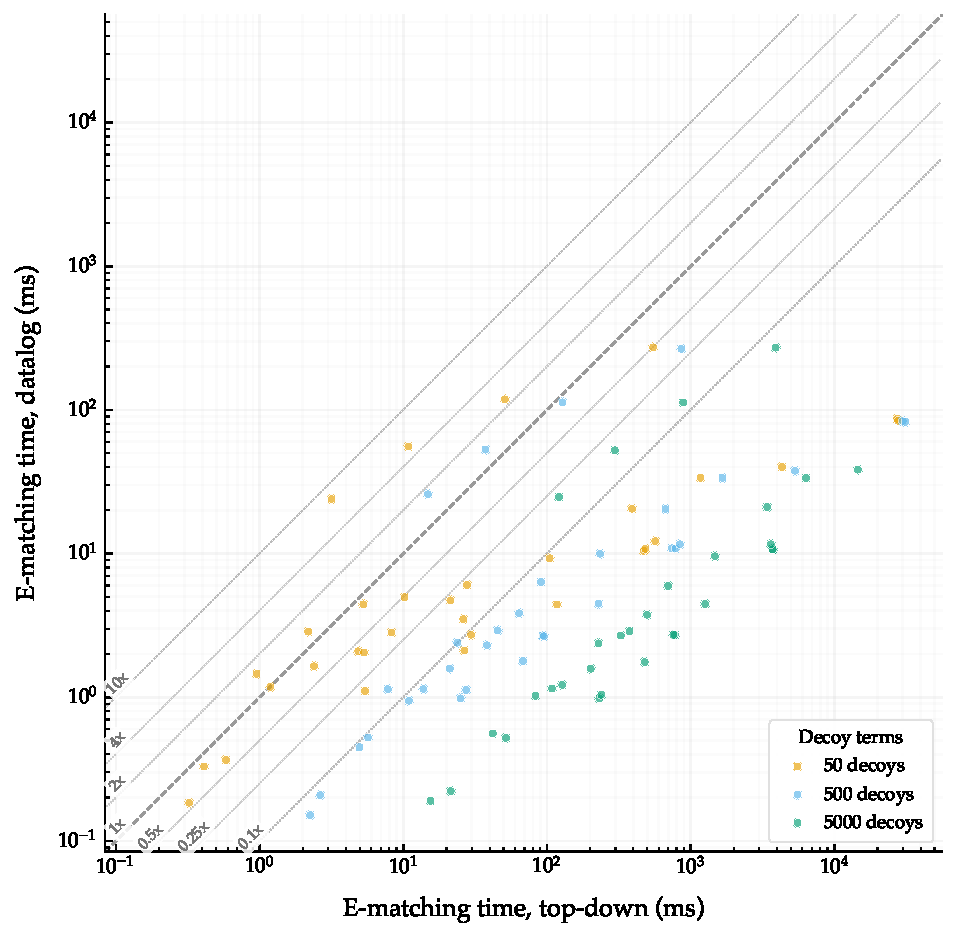
\includegraphics[width=\linewidth]{figs/matcher_cost_synthetic.pdf}
    \caption{Synthetic benchmarks.}
    \label{fig:matcher-cost-synthetic}
  \end{subfigure}\hfill
  \begin{subfigure}[t]{0.48\textwidth}
    \centering
    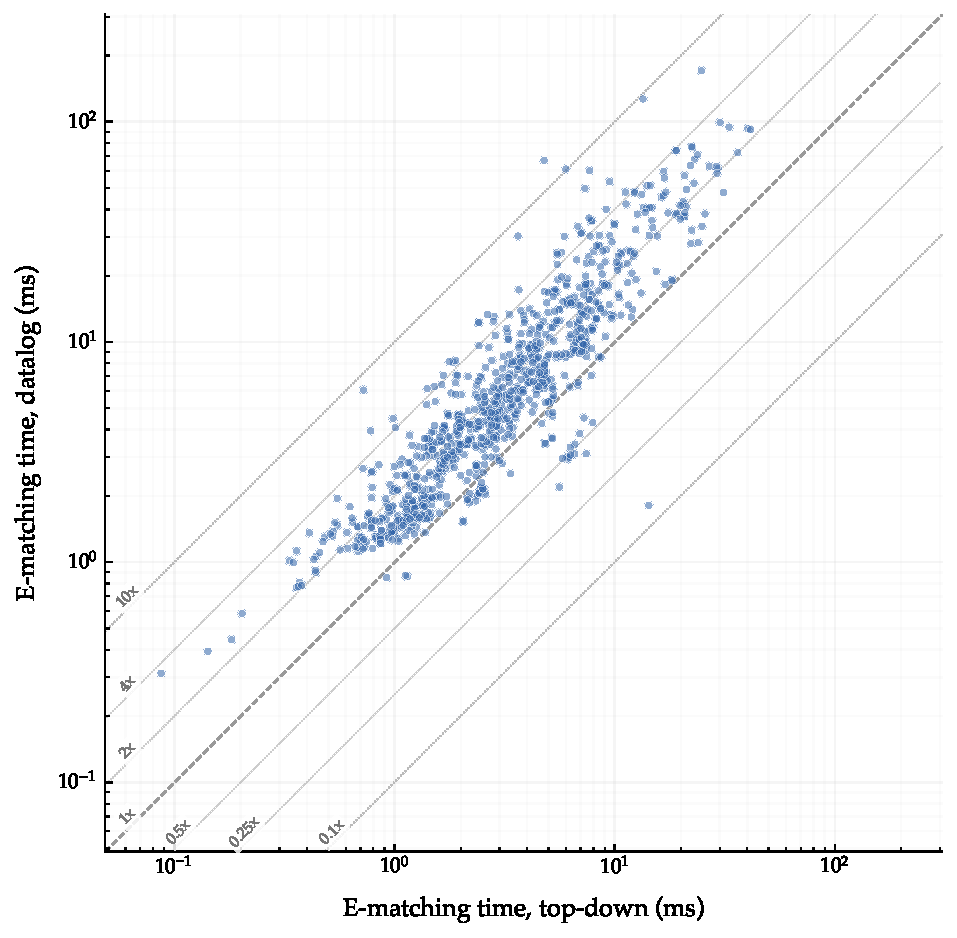
\includegraphics[width=\linewidth]{figs/matcher_cost_verus.pdf}
    \caption{Verus benchmarks.}
    \label{fig:matcher-cost-verus}
  \end{subfigure}
  \caption{Per-query e-matching time, top-down (x-axis) versus relational
  (y-axis), in seconds. Points below the diagonal are queries on which
  relational e-matching is faster. Left: synthetic benchmarks designed to
  stress nested patterns. Right: queries from the Verus program verifier.}
  \label{fig:matcher-cost}
\end{figure*}

We focus on e-matching time in isolation, rather than end-to-end solve time as
our current relational e-matching implementation is a prototype with significant
overhead from the \texttt{im::OrdMap} data structure. Thus, given a 60s timeout,
we the relation e-matching approach solves 96 queries (75 \%) on synthetic
benchmarks and 2247 queries (59.7 \%) on Verus benchmarks, while the top-down
approach solves 123 queries (96.1 \%) on synthetic benchmarks and 2414 queries (64.2
\%) on Verus benchmarks. We discuss the end-to-end picture in more detail in
Section~\ref{sec:conclusion}.

\subsection{Synthetic benchmarks}

The synthetic suite is a parameterized generalization of the running example
from Section~\ref{sec:background}. Each query uses a nested trigger similar to
\smt{g(h(x), x)}, but could also vary in the number 

We populate the e-graph with a varying number of
\emph{decoy} entries: extra ground assertions of the form \smt{(g d_i d_i)}
that add to the \smt{g}-table without contributing to any match. The number
of decoys is the principal axis of variation; a smaller axis varies the size
of the \smt{h}-table. Decoys exercise precisely the asymmetry that
distinguishes the two algorithms: top-down e-matching must scan every
\smt{g}-entry (decoys included) to find candidates, whereas relational
e-matching starts from the comparatively small \smt{h}-table and
index-joins into \smt{g}, touching only the relevant entries. The suite is
therefore designed to reward the relational approach as the decoy count
grows.

On this suite, relational e-matching is dramatically faster than top-down
e-matching. Of the 94 queries solved by both matchers, relational e-matching is
faster on 87, with a median speedup of $25\times$ ($2.92\times$ mean). Additionally,
the speedup grows with the number of decoys, as expected. 

\subsection{Verus benchmarks}

 Restricting attention to
the $n = 908$ queries that complete within one second under both matchers
, top-down e-matching is faster on
average, with a median ratio of $1.77\times$ (mean $2.04\times$)
in favor of top-down; relational e-matching is faster on only $53$ of the
$908$ queries.

These results suggest that more work is needed to realize the asymptotic
advantage of relational e-matching does not translate directly into a practical
win on real workloads. Closing this gap is the central engineering challenge
identified in Section~\ref{sec:conclusion}.

\section{Related Work}
\label{sec:related}

\paragraph{E-graphs and congruence closure.}
The e-graph data structure was introduced by Greg Nelson in his 1980 PhD
thesis~\cite{nelson1980}, alongside the congruence-closure decision procedure
developed jointly with Derek Oppen~\cite{nelsonoppen}. The e-graph was originally
designed as the core data structure of the simplifier in the Stanford Pascal
Verifier, where it represented equivalence classes of ground terms under the
axioms of equality and uninterpreted functions. Modern SMT solvers and
equality saturation engines inherit this design.

\paragraph{E-matching in theorem provers.}
The idea of \emph{matching modulo the equivalence stored in the e-graph} --- now
called e-matching --- already appears in Nelson's thesis~\cite{nelson1980} . The
technique was refined and used in the ESC line of program checkers, but its
first detailed algorithmic exposition is the canonical Simplify paper of
Detlefs, Nelson, and Saxe~\cite{simplify}. Our work targets the same problem ---
finding all matches of a pattern modulo an e-graph --- but compares Simplify's
recursive top-down matcher with a relational e-matching algorithm.

\paragraph{Indexing for SMT e-matching.}
de Moura and Bj{\o}rner introduced the \emph{e-matching code tree}, a
compiled abstract matching machine that shares prefix work across many
patterns simultaneously, and the \emph{inverted path index}, which makes
e-matching incremental as the e-graph grows~\cite{ematchingz3}. A companion
paper~\cite{ematchingfunprofit} surveys the practical lessons from deploying
these techniques in Z3 and motivates index-based matching as the workhorse of
modern SMT quantifier instantiation. Code trees are the closest prior work to
our approach in spirit: both compile patterns to a more efficient
representation than naive top-down traversal. The key difference is that code
trees still drive matching from the pattern root, whereas relational
e-matching is free to start from whichever relation is smallest.

\paragraph{Equality saturation.}
Equality saturation, introduced by Tate et al.~\cite{eqsat}, repurposes the
e-graph as a compiler intermediate representation: rewrite rules are applied to
saturation and an optimal program is then extracted, sidestepping the
phase-ordering problem in traditional optimizers. The egg library~\cite{egg}
made this approach widely practical by introducing deferred rebuilding of
congruence invariants and e-class analyses. Relational
e-matching~\cite{relationalematching} was developed in this lineage and
implemented in egglog~\cite{egglog}, where the absence of backtracking makes
maintaining the relational indices straightforward. Our contribution is to push
these ideas back into the SMT setting, where backtracking is unavoidable and the
index structures must be made backtrackable. Another difference is that egglog 
employs a worst-case optimal join algorithm~\cite{wcoj}, whereas our current implementation uses a
left-deep binary join. We leave the implementation of a worst-case optimal
join for future work.

\section{Conclusion and Future Work}
\label{sec:conclusion}

We have presented an initial implementation of relational e-matching inside an
SMT solver, identifying \emph{backtracking} as the central obstacle. Our
synthetic benchmarks demonstrate that the relational approach can substantially
outperform the conventional top-down matcher. Our results on Verus benchmarks
suggest that it is not that simple to translate this asymptotic advantage into a
practical win on real workloads. Closing the remaining gap will require a
combination of better data structures, better query planning, and a tighter
integration with the rest of the solver. We sketch the most promising directions
below.

\paragraph{Better backtrackable index maps.}
Our current implementation maintains
indices as persistent maps, which is correct but leaves substantial performance
on the table. Other datastructures are backtracked using trail-based undo logs, or
amortized rebuilding schemes. Bringing these to bear on the
relational indices would directly translate into reduced per-decision overhead.

\paragraph{Understanding what real benchmarks need.}
Synthetic benchmarks let us showcase the asymptotic advantage of relational
e-matching. We do not yet
have a precise characterization of which patterns and which workloads benefit,
and which do not. A more careful study --- profiling pattern shapes, e-graph sizes,
and the distribution of trigger applications across decision levels --- is needed.

\paragraph{Multi-query optimization.}
Today our implementation compiles each trigger into its own query plan and
runs each plan independently. SMT solvers, however, evaluate hundreds or
thousands of triggers against the same e-graph; many of these triggers share
sub-patterns. The database community has long studied multi-query optimization,
and Z3's code trees~\cite{ematchingz3} can be viewed as exactly this kind of
sharing applied to top-down e-matching. We expect that a relational analogue
--- sharing common sub-joins across triggers, or jointly planning batches of
triggers --- would yield substantial savings on real workloads.

\paragraph{Heuristics inside the query planner.}
Relational e-matching opens the door to a much richer space of optimizations
than top-down matching, because the planner now has visibility into what work
will be done. Many SMT-specific heuristics fit naturally into this framework.
For instance, \emph{relevancy filtering}~\cite{relevancy} --- restricting
matches to terms the SAT engine currently considers active --- can be
expressed as an additional selection in the join plan, and a planner that
knows about relevancy can prune entire join paths early. Other heuristics, such as preferring patterns
that have produced useful instantiations in the past, or biasing the join
order toward terms involved in recent conflicts, similarly fit as cost-model
inputs to the planner.

% \paragraph{Outlook.}
Indexing techniques have proven helpful in SMT
performance: code trees and inverted path indices~\cite{ematchingz3} are widely
credited with making large-scale e-matching tractable in Z3. Relational
e-matching is, in a precise sense, the most general indexing technique
available --- it subsumes pattern compilation as a special case and grants the
planner full freedom to reorder and share work. With backtrackability solved
and the right query-planning heuristics in place, we believe relational
e-matching has a real path to becoming a practical and broadly useful
component of modern SMT solvers.


\bibliographystyle{ACM-Reference-Format}
\bibliography{refs}

\end{document}
